\subsection{Момент вылета электрона из скрещенных полей}

Обозначим длину пластин $L$. Из уравнения (\ref{dv}) ($\frac{dv_z}{dt}=0$) следует, что скорость $v_z$ постоянна. Тогда время $\tau$ пролета сквозь пластины будет выражаться как:
\begin{equation}
	\tau=\frac{L}{v_z}
\end{equation}

Запишем формулу ларморовского радиуса, по которому электрон будет обращаться по вылете из пластин:
\begin{equation}
	r=\frac{mv_\perp}{eB}=\frac{v_\perp}{\eta{B}}=\frac{v_\perp}{\omega}
\end{equation}

Где 
\begin{equation}
	v_\perp=\sqrt{v_y(\tau)^2+v_x(\tau)^2}
\end{equation}

Итак, можем считать известными координаты и модуль скорости (в плоскости $XY$) электрона. 
Найдем направление скорости:
\begin{equation}
	\label{eq:tg_a}
	\tg{\alpha}=\left|\frac{v_x(\tau)}{v_y(\tau)}\right|=\left|\frac{\sin{\omega{\tau}}}{\cos\omega{\tau}-1}\right|
\end{equation}


% \begin{figure}[ht!]
% 	\centering
% 	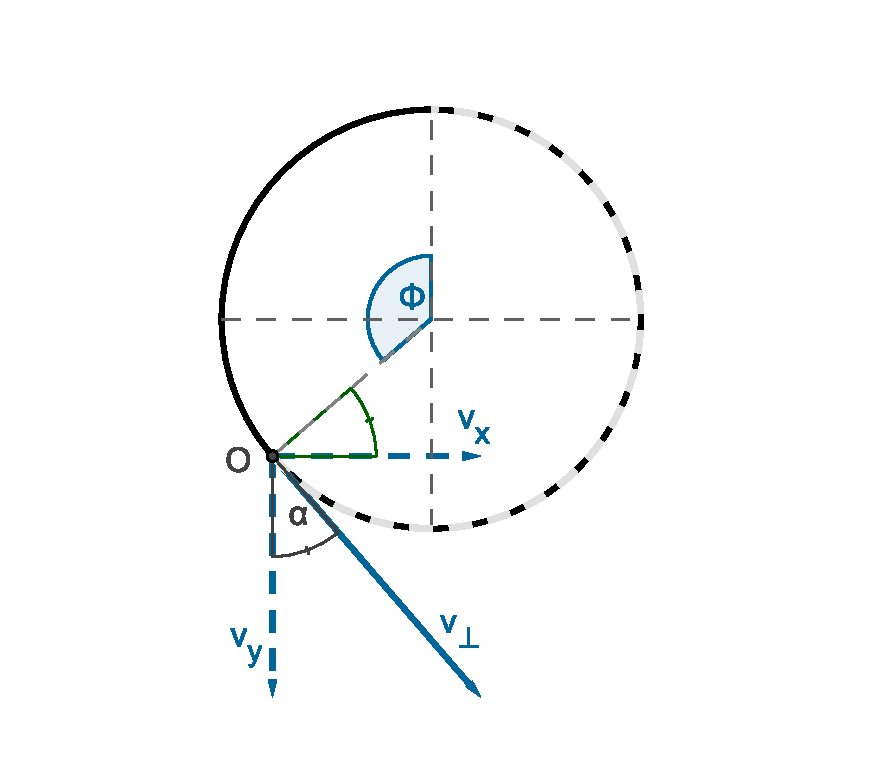
\includegraphics[width=0.65\textwidth]{figure_3.eps}
% 	\caption{Вылет электрона из скрещенных полей в точке O}
% 	\label{fig:figure1}
% \end{figure}

\begin{figure}[ht!]
\vspace{1cm}
\centering
\begin{minipage}[ht!]{0.49\linewidth}
\center{\includegraphics[width=0.9\linewidth]{o_horisontal} \\ а) горизонтально отклоняющие пластины}
\end{minipage}
\hfill
\begin{minipage}[ht!]{0.49\linewidth}
\center{\includegraphics[width=0.9\linewidth]{o_vertical} \\ б) вертикально отклоняющие пластины}
\end{minipage}
\vspace{0.5cm}
\caption{Вылет электрона из скрещенных полей в точке O.}
\vspace{1cm}
\label{ris:vert_hor}
\end{figure}

Также отметим, что электрическое поле является низкочастотным, и за время пролета частицы в нем поле можно считать постоянным. Тогда применимы формулы (\ref{eq:diff_dvx2}$\div$\ref{eq:tg_a}).

Отсюда следует что угол, под которым вылетает электрон из скрещенных полей от текущего напряжения $E(\tau)$ на пластинах не зависит. 

От напряжения зависит модуль скорости, а значит, и величина ларморовского радиуса. 

Вылетая из скрещенных полей в момент времени $\tau$, электрон летит со скоростью $v_\perp$ в плоскости $XY$ и под действием магнитного поля вращается по окружности (также в плоскости $XY$)

Мгновенный центр окружности при $t=\tau$ будет лежать на нормали к вектору скорости.

Тогда можно найти угол $\Phi$ -- угол поворота, набранный в скрещенных полях, из геометрии траектории - это будет $$\Phi=\frac{\pi}{2}+\alpha$$

Мы рассмотрели случай для горизонтально отклоняющих пластин ($E=E_x$). Понятно, что для вертикально отклоняющих пластин уравнения почти не изменятся: оси повернутся на $\frac{\pi}{2}$ (угол $\Phi$ будет острым), а $\tg{\alpha}$ поменяется на $\ctg{\alpha}$.

Таким образом, для горизонтально отклоняющих пластин 

\begin{gather}
	\tg{\alpha_2}=\left|\frac{v_y(\tau)}{v_x(\tau)}\right|=\left|\frac{\cos\omega{\tau}-1}{\sin{\omega{\tau}}}\right|=\frac{1}{\tg{\alpha}}=\ctg{\alpha}\\
	\Phi=\arctg{(\ctg{\alpha})}=\frac{\pi}{2}-\arcctg{(\ctg{\alpha})}=\frac{\pi}{2}-\alpha
\end{gather}

Число фокусировок можно определить как $n=\frac{\gamma}{2\pi}$, где $\gamma$ -- весь набранный электроном угол.

Тогда
\begin{equation}
	n=\frac{\Phi+\omega\frac{l}{v_z}}{2\pi}
\end{equation}
где $l$ -- расстояние от конца пластин до экрана.

Расчеты приведены в таблице ниже.

\begin{table}[ht!]
\begin{center}
\begin{tabular}{|c|c|c|c|c|c|c|}

\hline
$U_a$, В & $I_1$, А & $I_2$, А & $\alpha$, рад & $n$, эксперимент & $\Delta{n}$ & $n$, теория\\
\hline
$1200$ & $0.6$ 	& $1.14$ & $1.193$ 	& $1.11$ & $0.1$  	& $1.21$ \\ \hline
$1000$ & $0.54$ & $1.04$ & $1.198$ 	& $1.08$ & $0.1$ 	& $1.15$ \\ \hline
$1000$ & $0.5$ 	& $1.08$ & $1.176$ 	& $0.86$ & $0.07$  	& $0.94$ \\ \hline
$1100$ & $0.46$ & $1.08$ & $1.225$	& $0.74$ & $0.07$ 	& $0.81$ \\ \hline
\end{tabular}
\end{center}
\caption{\label{tab:n1n2}Расчет фокусировок двумя методами}
\end{table} 
